\documentclass{article}
%%%%%%%%%%%%%%%%%%%%%%%%%%%%% Define Article %%%%%%%%%%%%%%%%%%%%%%%%%%%%%%%%%%
%%%%%%%%%%%%%%%%%%%%%%%%%%%%%%%%%%%%%%%%%%%%%%%%%%%%%%%%%%%%%%%%%%%%%%%%%%%%%%%

%%%%%%%%%%%%%%%%%%%%%%%%%%%%% Using Packages %%%%%%%%%%%%%%%%%%%%%%%%%%%%%%%%%%
\usepackage{float}
\usepackage[letterpaper,portrait]{geometry}
\usepackage{graphicx}
\usepackage{anysize}
\usepackage{lipsum}
\usepackage{amsmath,amssymb,amsthm}
\usepackage[utf8]{inputenc}
\usepackage{multirow}
\usepackage{csquotes}
\usepackage[spanish]{babel}
\usepackage{apacite}
\usepackage{multicol}
\usepackage{parskip}
\usepackage{setspace}
\usepackage{empheq}
\usepackage{mdframed}
\usepackage{booktabs}
\usepackage{lipsum}
\usepackage{graphicx}
\usepackage{color}
\usepackage{psfrag}
\usepackage{pgfplots}
\usepackage{bm}
\usepackage{tocloft}
\usepackage{lscape}
\usepackage{adjustbox}
\setlength{\tabcolsep}{1.505625pt}
\renewcommand{\arraystretch}{1.2}
%%%%%%%%%%%%%%%%%%%%%%%%%%%%%%%%%%%%%%%%%%%%%%%%%%%%%%%%%%%%%%%%%%%%%%%%%%%%%%%

% Other Settings

%%%%%%%%%%%%%%%%%%%%%%%%%% Page Setting %%%%%%%%%%%%%%%%%%%%%%%%%%%%%%%%%%%%%%%
\geometry{letterpaper, margin=2.54cm}

%%%%%%%%%%%%%%%%%%%%%%%%%% Define some useful colors %%%%%%%%%%%%%%%%%%%%%%%%%%
\definecolor{ocre}{RGB}{243,102,25}
\definecolor{mygray}{RGB}{243,243,244}
\definecolor{deepGreen}{RGB}{26,111,0}
\definecolor{shallowGreen}{RGB}{235,255,255}
\definecolor{deepBlue}{RGB}{61,124,222}
\definecolor{shallowBlue}{RGB}{235,249,255}
%%%%%%%%%%%%%%%%%%%%%%%%%%%%%%%%%%%%%%%%%%%%%%%%%%%%%%%%%%%%%%%%%%%%%%%%%%%%%%%

%%%%%%%%%%%%%%%%%%%%%%%%%% Define an orangebox command %%%%%%%%%%%%%%%%%%%%%%%%
\newcommand\orangebox[1]{\fcolorbox{ocre}{mygray}{\hspace{1em}#1\hspace{1em}}}
%%%%%%%%%%%%%%%%%%%%%%%%%%%%%%%%%%%%%%%%%%%%%%%%%%%%%%%%%%%%%%%%%%%%%%%%%%%%%%%

%%%%%%%%%%%%%%%%%%%%%%%%%%%% English Environments %%%%%%%%%%%%%%%%%%%%%%%%%%%%%
\newtheoremstyle{mytheoremstyle}{3pt}{3pt}{\normalfont}{0cm}{\rmfamily\bfseries}{}{1em}{{\color{black}\thmname{#1}~\thmnumber{#2}}\thmnote{\,--\,#3}}
\newtheoremstyle{myproblemstyle}{3pt}{3pt}{\normalfont}{0cm}{\rmfamily\bfseries}{}{1em}{{\color{black}\thmname{#1}~\thmnumber{#2}}\thmnote{\,--\,#3}}
\theoremstyle{mytheoremstyle}
\newmdtheoremenv[linewidth=1pt,backgroundcolor=shallowGreen,linecolor=deepGreen,leftmargin=0pt,innerleftmargin=20pt,innerrightmargin=20pt,]{theorem}{Theorem}[section]
\theoremstyle{mytheoremstyle}
\newmdtheoremenv[linewidth=1pt,backgroundcolor=shallowBlue,linecolor=deepBlue,leftmargin=0pt,innerleftmargin=20pt,innerrightmargin=20pt,]{definition}{Definition}[section]
\theoremstyle{myproblemstyle}
\newmdtheoremenv[linecolor=black,leftmargin=0pt,innerleftmargin=10pt,innerrightmargin=10pt,]{problem}{Problem}[section]
%%%%%%%%%%%%%%%%%%%%%%%%%%%%%%%%%%%%%%%%%%%%%%%%%%%%%%%%%%%%%%%%%%%%%%%%%%%%%%%

%%%%%%%%%%%%%%%%%%%%%%%%%%%%%%% Plotting Settings %%%%%%%%%%%%%%%%%%%%%%%%%%%%%
\usepgfplotslibrary{colorbrewer}
\pgfplotsset{width=8cm,compat=1.9}
%%%%%%%%%%%%%%%%%%%%%%%%%%%%%%%%%%%%%%%%%%%%%%%%%%%%%%%%%%%%%%%%%%%%%%%%%%%%%%%

%%%%%%%%%%%%%%%%%%%%%%%%%%%%%%% Title & Author %%%%%%%%%%%%%%%%%%%%%%%%%%%%%%%%
\author{Gustavo Vergara}
%%%%%%%%%%%%%%%%%%%%%%%%%%%%%%%%%%%%%%%%%%%%%%%%%%%%%%%%%%%%%%%%%%%%%%%%%%%%%%%

\begin{document}
\pgfplotsset{compat=1.18}
\setstretch{2}

\begin{titlepage}
	\centering
	\vspace{2.5cm}
	{\scshape \Large TALLER HERRAMIENTAS DE CONTROL \par}
	\vspace{5cm}
	\textbf\large\scshape{\par}
	\vspace{0.5cm}

	{\Large Vergara Pareja Gustavo\par}
	\vspace{5cm}
	{\scshape\Large Miguel Ángel Lancheros\par}
	\vspace{0.3cm}
	{\scshape\Large Metrología y Control de Calidad - G1IM \par}
	\vspace{0.3cm}
	{\scshape\Large Universidad de Córdoba\par}
	\vspace{0.3cm}
	{\Large 6 de Diciembre de 2023 \par}
\end{titlepage}
%\tableofcontents
\newpage

\section{Espina de pescado (Causa y efecto)}
El análisis de causa y efecto, también
llamado diagrama de espina de
pescado o diagrama de Ishikawa, es
una herramienta que se utiliza para
identificar las posibles causas de un
problema específico. Fue
desarrollado por el ingeniero japonés
Kaoru Ishikawa en la década de 1960
y se utiliza ampliamente en la
resolución de problemas y en la
mejora de la calidad.
\begin{enumerate}
	\item ¿Como se presenta?\newline
	El diagrama de Ishikawa se presenta
	como una especie de espinas de
	pescado, de ahí su nombre, donde el
	eje horizontal representa el problema
	que se está analizando y el eje vertical
	representa las posibles causas que
	pueden estar contribuyendo al
	problema. Las espinas son líneas que
	se extienden desde el eje horizontal y
	se conectan con las costillas, que
	representan las diferentes categorías
	de causas.   
		            \begin{figure}[H]
			            \centering
			            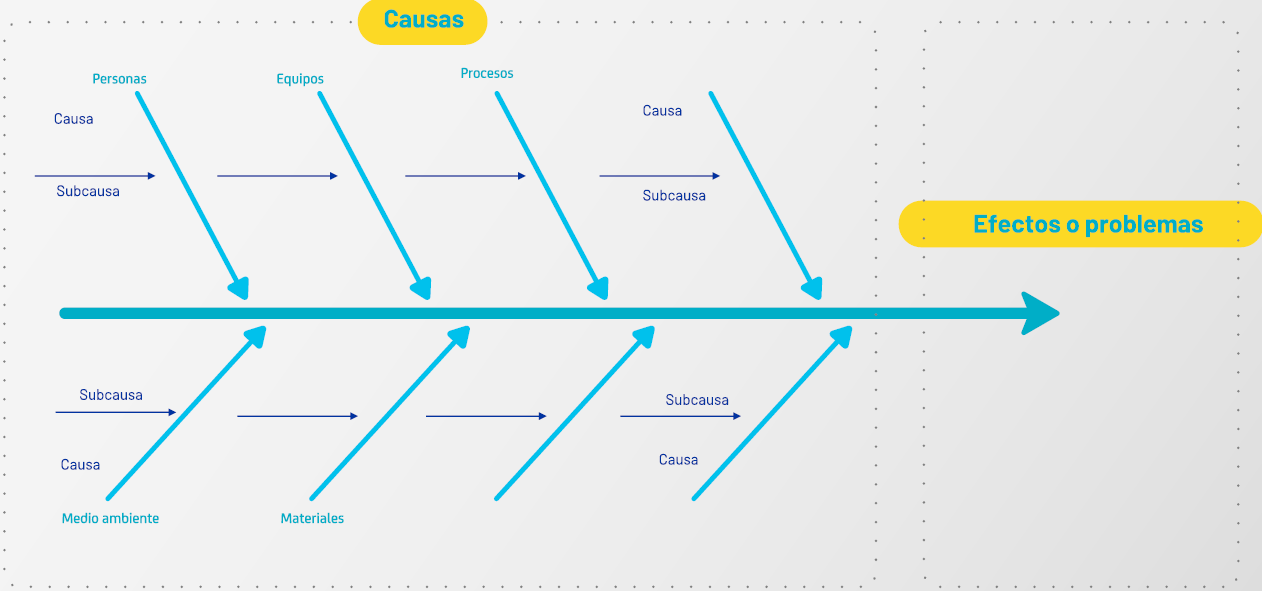
\includegraphics[width=1\textwidth]{espina.png}
			            \caption{Espina de pescado}
			            \label{fig:imagen2}
		            \end{figure}
	\item ¿Para qué sirve la
	metodología de análisis
	de causa-efecto en una
	organización?\newline
	El análisis de causa-efecto es una
	herramienta muy útil en las
	organizaciones debido a que permite
	identificar y analizar las posibles
	causas de un problema o una situación,
	a continuación se describen las
	utilidades de la metodología en una
	organización.
	      \begin{itemize}
			\newpage
		      \item Identificación de las causas de un problema\newline
		      El análisis de causa-efecto ayuda a las organizaciones a identificar las causas subyacentes de un problema en particular. Al hacer esto, se puede desarrollar una mejor comprensión del problema y se pueden tomar medidas para abordarlo adecuadamente.
				\item Mejora continua\newline
				Al utilizar el análisis de causa-efecto para identificar las causas de un problema, las organizaciones pueden desarrollar planes de mejora continua. Esto implica identificar y eliminar las causas raíz de los problemas para mejorar los procesos y las operaciones de la organización.
				\item Resolución de problemas\newline
				Al analizar las causas subyacentes de un problema, el análisis de causa-efecto ayuda a las organizaciones a desarrollar soluciones efectivas para resolver el problema. Estas soluciones se enfocan en abordar las causas raíz y no solo los síntomas del problema.
				\item Planificación y toma de decisiones\newline
				El análisis de causa-efecto se utiliza comúnmente en la planificación y toma de decisiones. Las organizaciones pueden utilizarlo para identificar los factores que afectan los resultados y, por lo tanto, tomar decisiones informadas para mejorar estos resultados.
			\end{itemize}
			\begin{figure}[H]
				\centering
				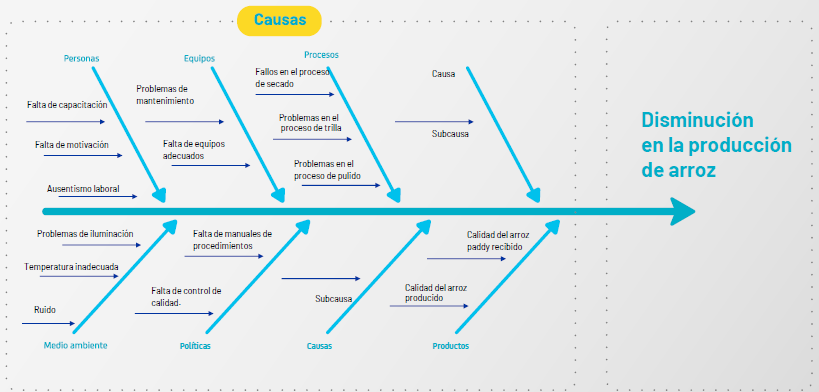
\includegraphics[width=1\textwidth]{espina2.png}
				\caption{Ejemplo de Espina de pescado}
				\label{fig:imagen2}
			\end{figure}
			\newpage

\section{Pareto}

El principio de Pareto es una herramienta de análisis y toma
de decisiones creada por Vilfredo Pareto (1848-1923)
a finales del siglo XIX en 1897. El economista y sociólogo
italiano, que estudió en la Universidad Politécnica de Turin en
ltalia, es considerado el padre fundador de lo que ahora se
llama "Principio de Pareto". Al estudiar la riqueza de su
país descubrió que sólo el 20\% de la gente poseía el 80\% de la
riqueza total. Luego aplicó esta ley a otros estados como
Rusia, Francia y Suiza y encontró los mismos resultados.
\begin{itemize}
	\item¿Comó surge el Principio de Pareto?
	      \begin{itemize}
		      \item El principio de Pareto surge de la observación de que el 20 \% de los clientes son responsables del 80\% de los efectos. Es decir en el mundo de los negocios, el 20 \% de los clientes son responsables del 80\% de la facturación. Al identificar este 20\% (los clientes más importantes) las empresas pueden prestarles más atención para ahorrar tiempo y dinero. Según Joseph Juran, el principio de Pareto se puede aplicar universalmente en el ámbito empresarial y se puede encontrar en todos los sectores de la sociedad. Incluso puedes utilizar el principio en la mayoría de las áreas de la vida diaria. Sin embargo, veremos que, tanto en el ámbito empresarial como en otros ámbitos, la relación 80/20 no siempre se respeta pero si da una idea de la realidad.
	      \end{itemize}
	\item El principio de Pareto como herramienta de control de calidad.\newline
	Una segunda aplicación, utilizada por Joseph Juran, es la del control
	y gestión de calidad en una línea de producción. Si el 20\% de
	Las fallas causan el 80\% de los problemas, la empresa puede concentrarse
	centrar sus esfuerzos en abordar las fallas en cuestión para
	para mejorar la calidad. También son válidas otras aplicaciones similares:
	\begin{itemize}
		\item El 20\% del tiempo de configuración de la máquina puede resolver el 80\% de los problemas;
		\item El 20\% de la línea de producción es responsable del 80\% del
		producto final.
	\end{itemize}
\newpage
	\item 	ESTUDIO DE CASO: UNA LÍNEA DE PRODUCCIÓN\newline
Introducción al problema\newline
Nuestro caso de estudio se refiere a una industria y su línea de
producción. En esta empresa, la línea de producción está
experimentando interrupciones recurrentes a lo largo del año. En conjunto
suman un total de 1033 horas, lo que supone poco más de un
mes de inactividad. Para compensar la pérdida de horas de trabajo,
el directivo, que advirtió que la dinámica no era lógica,
identifica las diez causas comunes de parada de línea. Luego estima
un tiempo de parada promedio (en horas) y proporciona un recuento
de ocurrencias para cada causa. Utilizando el principio de
Pareto, espera identificar los principales factores que perturban la línea
de producción.
\begin{table}[h!]
	\begin{tabular}{|l|l|l|l|l|}
	\hline 
	\multicolumn{1}{|p{155.83218pt}}{\raggedright Problemas (retraso en h)} & \multicolumn{1}{|p{61.730625pt}}{\raggedright Ocurrencias} & \multicolumn{1}{|p{48.18pt}}{\raggedright Total (h)} & \multicolumn{1}{|p{41.404686pt}}{\raggedright \%} & \multicolumn{1}{|p{60.225pt}|}{\raggedright Acumulado \ (\%)}\\ 
	\hline 
	\multicolumn{1}{|p{155.83218pt}}{\raggedright Configuraci\'on de la m\'aquina (7)} & \multicolumn{1}{|p{61.730625pt}}{\raggedright 56} & \multicolumn{1}{|p{48.18pt}}{\raggedright 392} & \multicolumn{1}{|p{41.404686pt}}{\raggedright 37,95} & \multicolumn{1}{|p{60.225pt}|}{\raggedright 37,95}\\ 
	\hline 
	\multicolumn{1}{|p{155.83218pt}}{\raggedright Recalibraci\'on (3)} & \multicolumn{1}{|p{61.730625pt}}{\raggedright 87} & \multicolumn{1}{|p{48.18pt}}{\raggedright 265} & \multicolumn{1}{|p{41.404686pt}}{\raggedright 25,27} & \multicolumn{1}{|p{60.225pt}|}{\raggedright 63,21}\\ 
	\hline 
	\multicolumn{1}{|p{155.83218pt}}{\raggedright Mala configuraci\'on (4)} & \multicolumn{1}{|p{61.730625pt}}{\raggedright 23} & \multicolumn{1}{|p{48.18pt}}{\raggedright 92} & \multicolumn{1}{|p{41.404686pt}}{\raggedright 8,91} & \multicolumn{1}{|p{60.225pt}|}{\raggedright 72,12}\\ 
	\hline 
	\multicolumn{1}{|p{155.83218pt}}{\raggedright Fuga de aceite de la m\'aquina (7)} & \multicolumn{1}{|p{61.730625pt}}{\raggedright 12} & \multicolumn{1}{|p{48.18pt}}{\raggedright 84} & \multicolumn{1}{|p{41.404686pt}}{\raggedright 8,13} & \multicolumn{1}{|p{60.225pt}|}{\raggedright 80,25}\\ 
	\hline 
	\multicolumn{1}{|p{155.83218pt}}{\raggedright Escasez de existencias (12)} & \multicolumn{1}{|p{61.730625pt}}{\raggedright 5} & \multicolumn{1}{|p{48.18pt}}{\raggedright 60} & \multicolumn{1}{|p{41.404686pt}}{\raggedright 5,81} & \multicolumn{1}{|p{60.225pt}|}{\raggedright 86,06}\\ 
	\hline 
	\multicolumn{1}{|p{155.83218pt}}{\raggedright Cambios de orden(4)} & \multicolumn{1}{|p{61.730625pt}}{\raggedright 15} & \multicolumn{1}{|p{48.18pt}}{\raggedright 60} & \multicolumn{1}{|p{41.404686pt}}{\raggedright 5,81} & \multicolumn{1}{|p{60.225pt}|}{\raggedright 91,87}\\ 
	\hline 
	\multicolumn{1}{|p{155.83218pt}}{\raggedright Fallo de compresor (7)} & \multicolumn{1}{|p{61.730625pt}}{\raggedright 4} & \multicolumn{1}{|p{48.18pt}}{\raggedright 28} & \multicolumn{1}{|p{41.404686pt}}{\raggedright 2,71} & \multicolumn{1}{|p{60.225pt}|}{\raggedright 94,58}\\ 
	\hline 
	\multicolumn{1}{|p{155.83218pt}}{\raggedright Huelga de empleados (24)} & \multicolumn{1}{|p{61.730625pt}}{\raggedright 1} & \multicolumn{1}{|p{48.18pt}}{\raggedright 24} & \multicolumn{1}{|p{41.404686pt}}{\raggedright 2,32} & \multicolumn{1}{|p{60.225pt}|}{\raggedright 96,90}\\ 
	\hline 
	\multicolumn{1}{|p{155.83218pt}}{\raggedright Corte de energ\'{\i}a (1)} & \multicolumn{1}{|p{61.730625pt}}{\raggedright 22} & \multicolumn{1}{|p{48.18pt}}{\raggedright 22} & \multicolumn{1}{|p{41.404686pt}}{\raggedright 2,13} & \multicolumn{1}{|p{60.225pt}|}{\raggedright 99,03}\\ 
	\hline 
	\multicolumn{1}{|p{155.83218pt}}{\raggedright Desglose general (2)} & \multicolumn{1}{|p{61.730625pt}}{\raggedright 5} & \multicolumn{1}{|p{48.18pt}}{\raggedright 10} & \multicolumn{1}{|p{41.404686pt}}{\raggedright 0,97} & \multicolumn{1}{|p{60.225pt}|}{\raggedright 100,00}\\ 
	\hline 
	\multicolumn{1}{|p{155.83218pt}}{\raggedright TOTAL} & \multicolumn{1}{|p{61.730625pt}}{\raggedright 230} & \multicolumn{1}{|p{48.18pt}}{\raggedright 1033} & \multicolumn{1}{|p{41.404686pt}}{\raggedright 100,00} & \multicolumn{1}{|p{60.225pt}|}{}\\ 
	\hline 
	
	\end{tabular}
	\end{table}	
	      \begin{figure}[H]
		      \centering
		      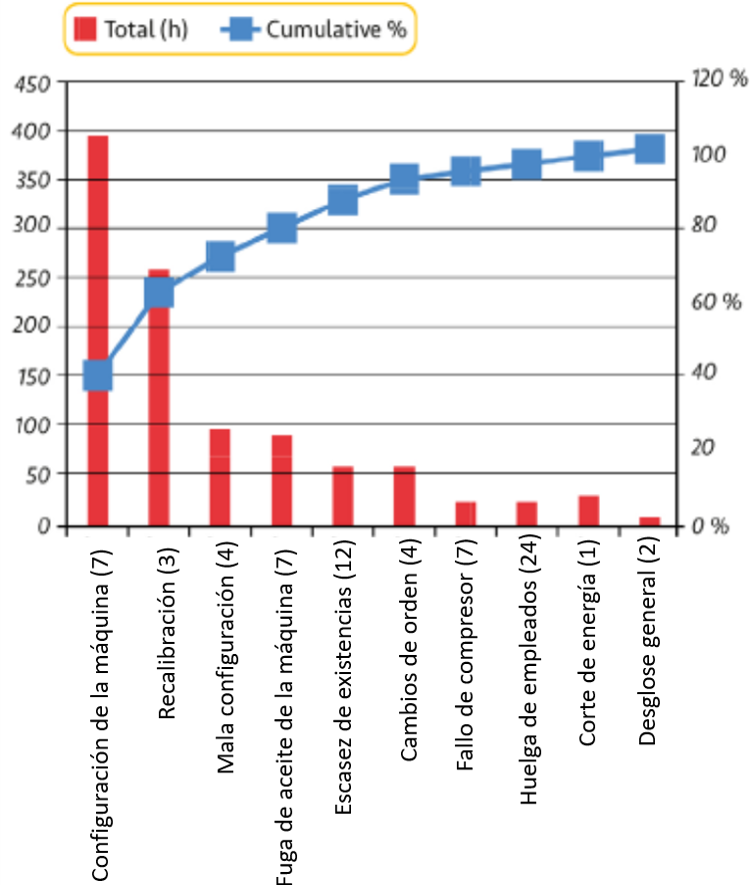
\includegraphics[width=0.7\textwidth]{Grapich.png}
		      \caption{Gráfico de la línea de producción de la industria}
		      \label{fig:imagen2}
	      \end{figure}

	\item Identificar los factores importantes\newline
	El principio de Pareto funciona particularmente bien en este caso
	porque una minoría de factores causa la mayoría de los problemas.
	En concreto, casi el 30\% de los factores provocan el 72\% de los retrasos
	en la línea de producción. Observe que hay otras dos proporciones
	cercanas a 80/20:
	      \begin{enumerate}
		      \item Al considerar las dos mayores causas (20\%), el
			  porcentaje de retrasos es del 63\%;
		      \item Si se consideran los cuatro mayores problemas (40\%), el
			  porcentaje de retrasos es del 80\%.
	      \end{enumerate}\newpage
		  \item ¿Cuál es la mejor proporción? \newline
		   Está claro que la proporción general del 30\% de los factores que
	causan el 72\% de los retrasos es la más cercana al principio de Pareto.
	Desafortunadamente, esto no resuelve todos los problemas:
	\begin{enumerate}
		\item En primer lugar, nos quedan muchos factores problemáticos
		que ajustar, pero elegir centrarnos en la primera proporción (dos
		cuestiones principales) nos centraríamos en una minoría de causas
		que causan el máximo número de consecuencias, que es precisamente
		el objetivo del principio de Pareto;
		\item En segundo lugar, si el director de la planta quiere solucionar tantos
		problemas como sea posible, tiene todos los motivos para centrarse en el
		tercer ratio, corrigiendo el 40\% de las causas que provocan el 80\% de
		los retrasos en la línea de producción.
	\end{enumerate}
		  \section{De flujo}
		  Muestran la secuencia de pasos y las posibilidades de ramificaciones que existen en un proceso que
		  transforma una o más entradas en una o más salidas. Los diagramas de flujo muestran las actividades,
		  los puntos de decisión, las ramificaciones, las rutas paralelas y el orden general de proceso.
		  En gestión de la calidad es una herramienta básica para la representación de los macroprocesos, procesos, subprocesos y/o tareas.
		  \begin{figure}[H]
			\centering
			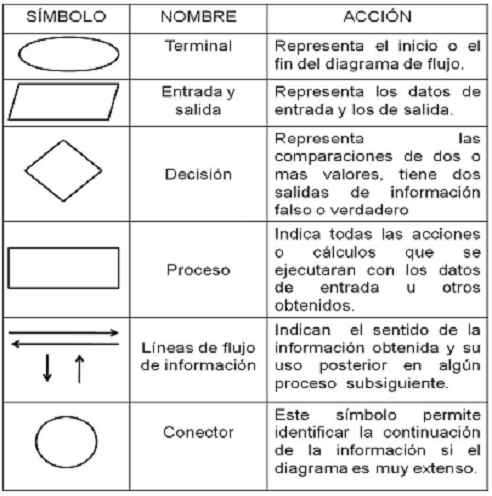
\includegraphics[width=0.4\textwidth]{flujo_simb.png}
			\caption{Simbología del diagrama de flujo}
			\label{fig:imagen2}
		\end{figure}
		Un diagrama de flujo presenta generalmente un único punto de inicio y un único punto de cierre, aunque puede tener más, siempre que cumpla con la lógica requerida.
		\begin{itemize}
			\item Pasos para construir un Diagrama de Flujo.
			\begin{enumerate}
				\item Definir el alcance del proceso a describir. De esta manera quedara fijado la entrada y la salida del diagrama.
				\item Identificar y enumerar las principales actividades/subprocesos que están incluidos en el proceso a describir.
				\item Establecer los puntos de decisión.
				\item Construir el diagrama respetando la secuencia cronológica y asignando los correspondientes símbolos.
				\item Fijar un título al diagrama y verificar que esté completo y describa con exactitud el proceso elegido.
			\end{enumerate}
		\end{itemize}  
		\begin{figure}[H]
			\centering
			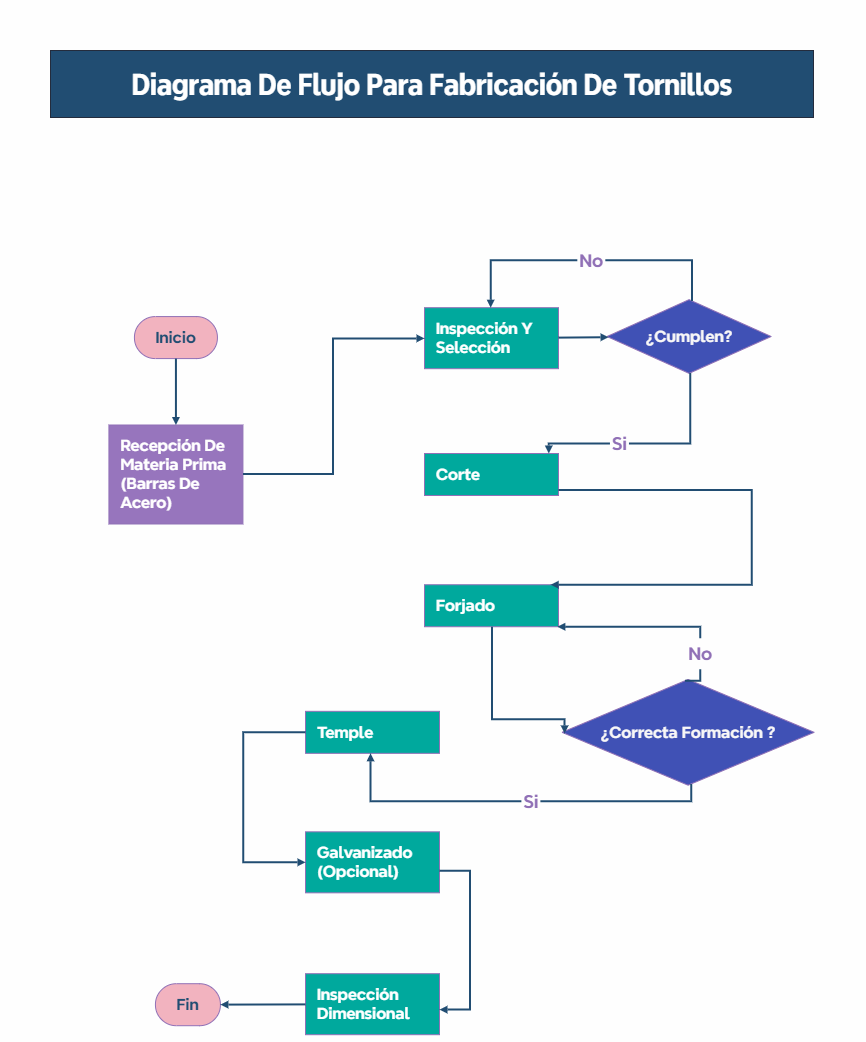
\includegraphics[width=\textwidth]{flujotornillos.png}
			\caption[short]{Ejemplo de diagrama de flujo}
			\label{fig:imagen2}
		  \end{figure}
		\section{Dispersión}
		\begin{itemize}
			\item Representan pares ordenados (X, Y) y a menudo se les denomina diagramas de correlación, ya que
			pretenden explicar un cambio en la variable dependiente. Y en relación con un cambio observado en la
			variable independiente X.\newline
			La dirección de la correlación puede ser proporcional (correlación positiva), inversa (correlación
			negativa), o bien puede no darse un patrón de correlación (correlación cero). En caso de que se pueda
			establecer una correlación, se puede calcular una línea de regresión y utilizarla para estimar cómo un
			cambio en la variable independiente influirá en el valor de la variable dependiente.
			\item Una empresa de fabricación de perfiles de acero se plantea cambiar la composición de uno de sus productos utilizando un nuevo carbono de una nueva empresa. Antes de tomar una decisión, la empresa decide realizar un ensayo para estudiar la posible relación entre la utilización dicha materia prima y el número de no conformidades. Para ello analiza lotes con diferentes porcentajes de la nueva materia prima y toma los siguientes datos:
			\begin{table}[H]
				\centering
				\begin{tabular}{|l|l|l|}
				\hline
					Nºmuestra & Porcentaje de carbono (\%) & Producto no conforme \\ \hline
					1 & 1 & 10 \\ \hline
					2 & 2 & 5 \\ \hline
					3 & 1.5 & 7 \\ \hline
					4 & 1.5 & 6 \\ \hline
					5 & 3 & 2 \\ \hline
					6 & 4 & 1 \\ \hline
					7 & 1.6 & 8 \\ \hline
					8 & 2.6 & 3 \\ \hline
					9 & 3.5 & 2 \\ \hline
					10 & 4.6 & 1 \\ \hline
					11 & 5 & 1 \\ \hline
					12 & 0.5 & 15 \\ \hline
					13 & 4.3 & 1 \\ \hline
					14 & 3.2 & 3 \\ \hline
					15 & 5.1 & 1 \\ \hline
					16 & 2.5 & 3 \\ \hline
					17 & 1.8 & 7 \\ \hline
					18 & 2.1 & 6 \\ \hline
					19 & 3.9 & 3 \\ \hline
					20 & 1.2 & 9 \\ \hline
					21 & 2.4 & 4 \\ \hline
					22 & 4.3 & 1 \\ \hline
					23 & 3.5 & 3 \\ \hline
					24 & 2.7 & 2 \\ \hline
					25 & 0.5 & 16 \\ \hline
					26 & 0.8 & 14 \\ \hline
					27 & 1.2 & 9 \\ \hline
					28 & 3.6 & 2 \\ \hline
					29 & 5.3 & 1 \\ \hline
					30 & 1 & 11 \\ \hline
				\end{tabular}
			\end{table}
		\end{itemize}
\end{itemize}
\begin{figure}[H]
	\centering
	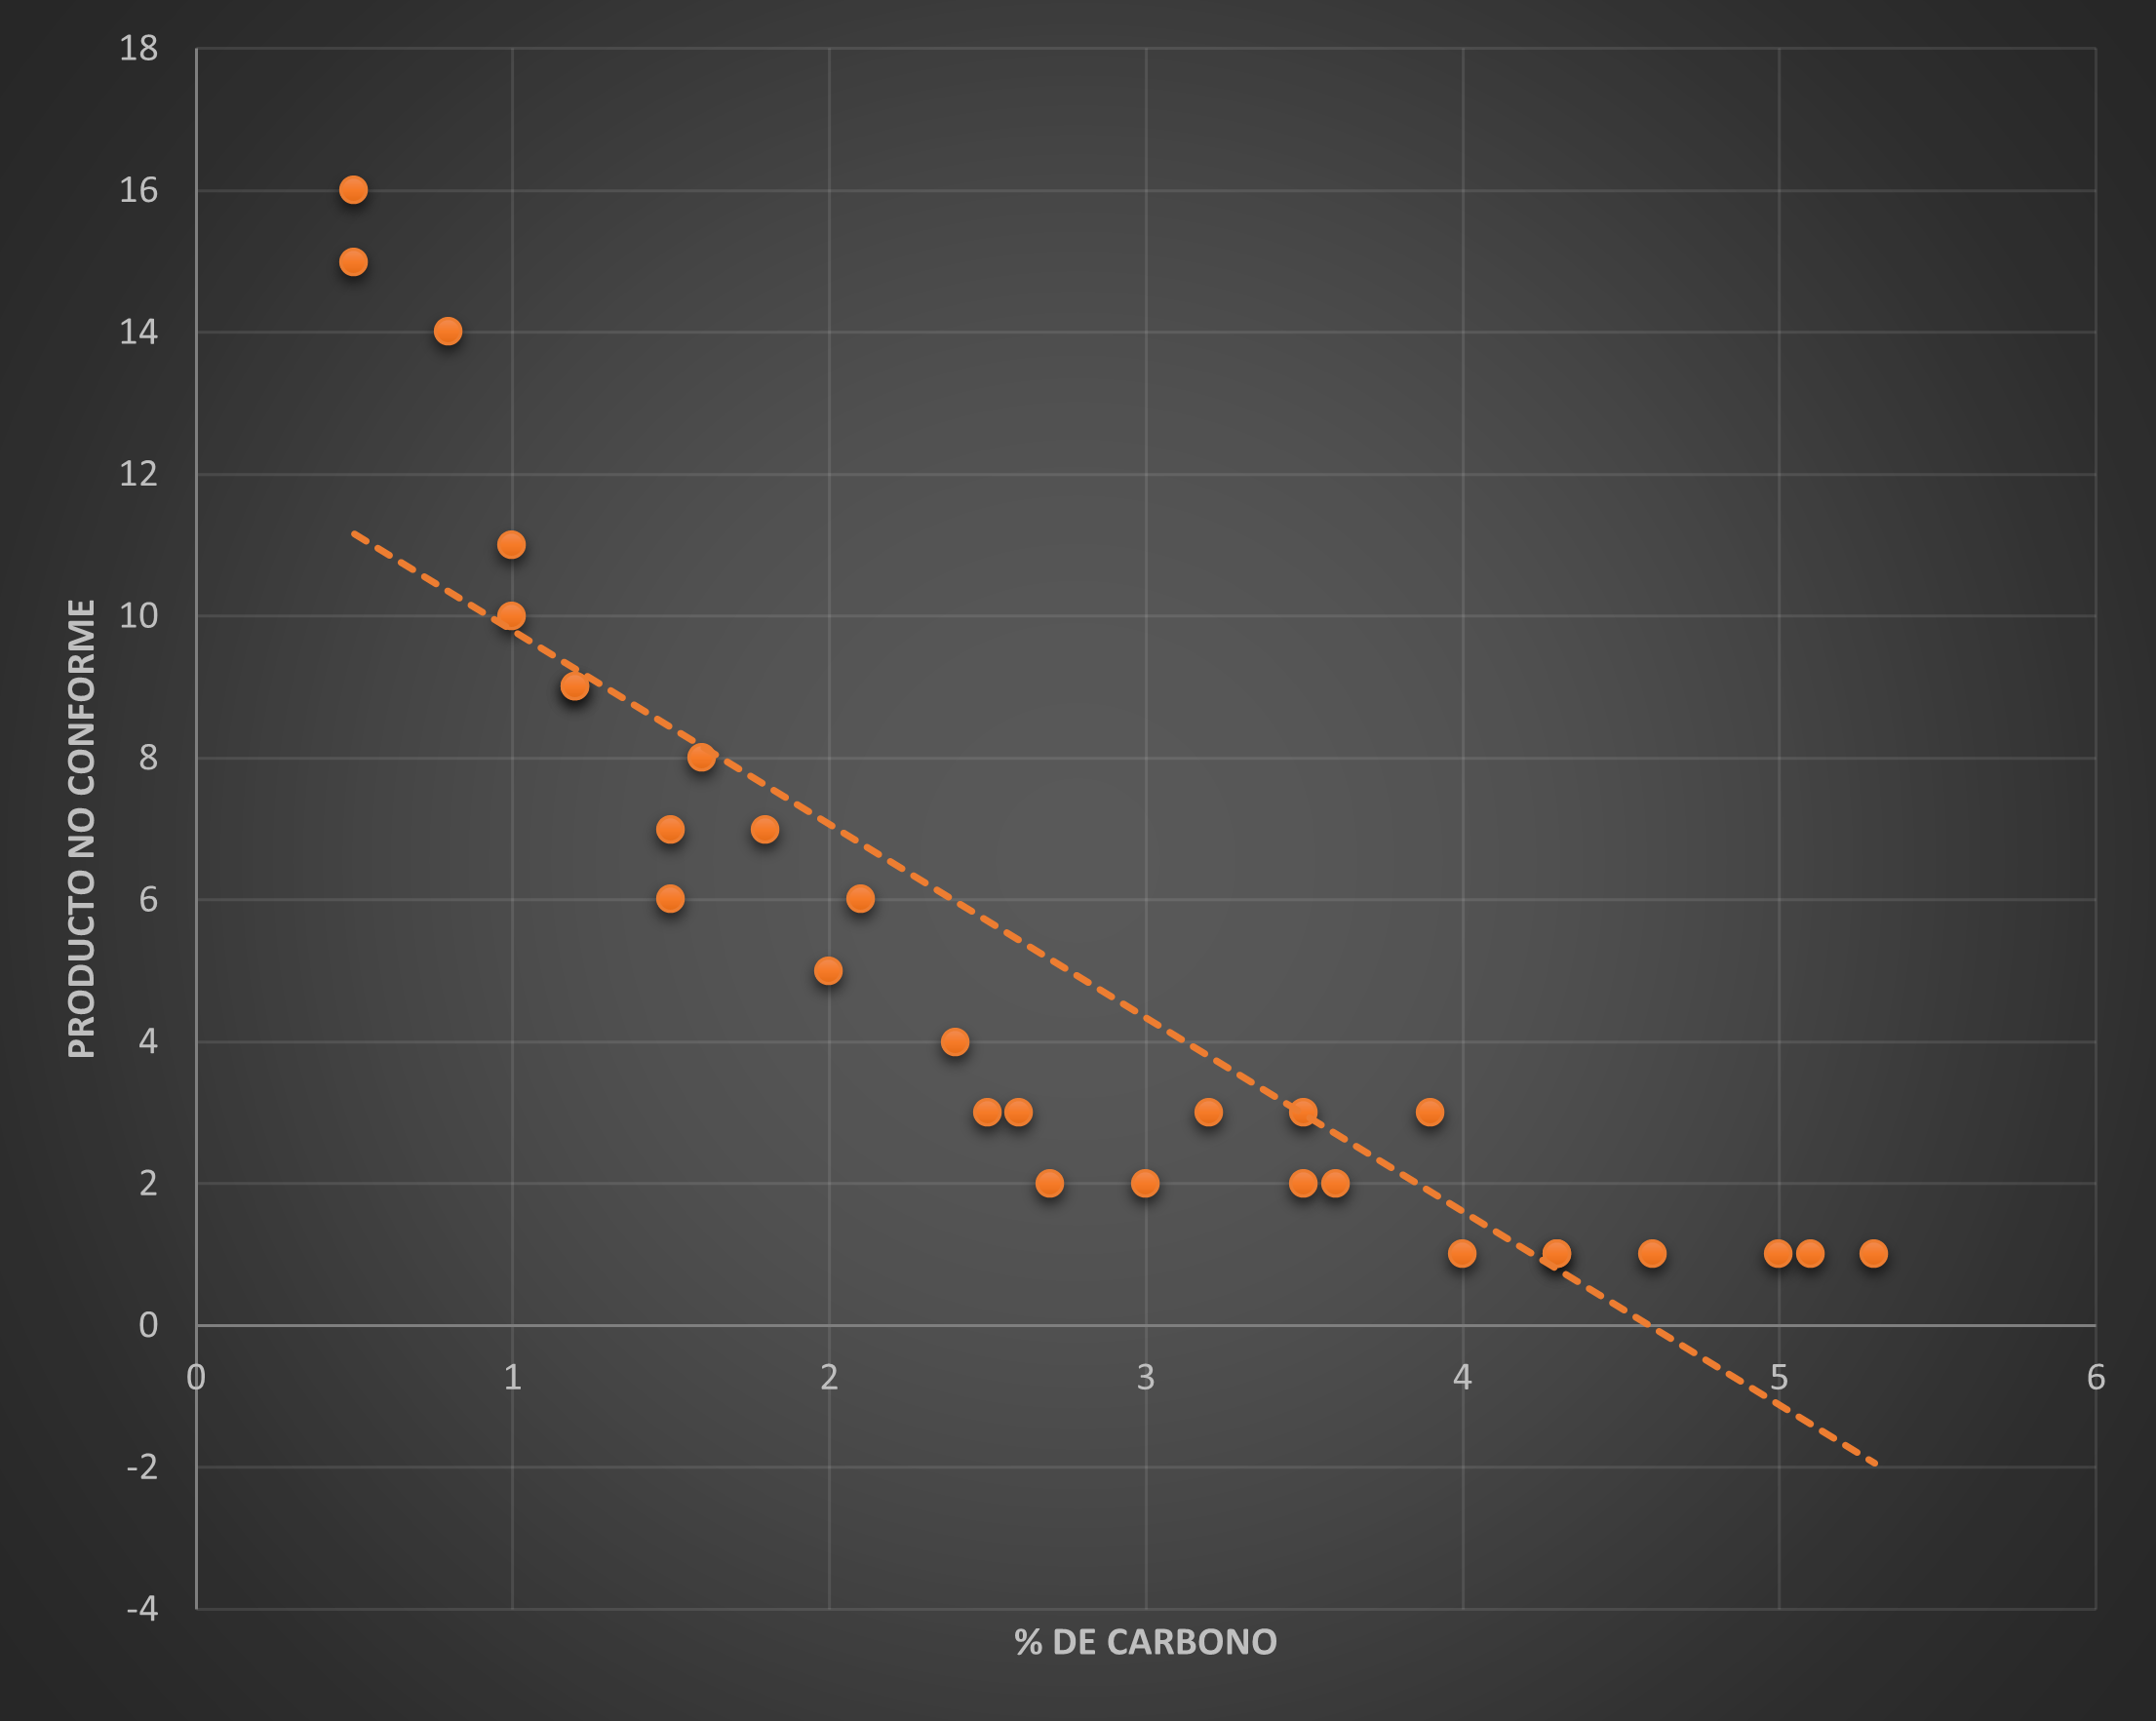
\includegraphics[width=\textwidth]{Dispersion1.png}
	\caption[short]{Gráfico de dispersión}
	\label{fig:imagen2}
  \end{figure}
  \begin{itemize}
	\item En este caso, tendremos una correlación negativa (a medida que aumentamos el \% de la nueva materia prima, disminuye el número de productos no conformes). Con estos resultados la empresa podría plantearse la introducción de la nueva materia prima, aunque debería combinarlo con otras herramientas para una mejor toma de decisiones.
  \end{itemize}\newpage
\section{Análisis de tendencia}


El análisis de tendencia es una técnica estadística que permite estudiar una o más variables en un período de tiempo aportando información para la toma de decisiones en la empresa.
Es muy demandado para observar la evolución de variables empresariales como las ventas o los costes. Así, las empresas necesitan conocer esta información para sobrevivir en mercados globales.
\begin{itemize}
	\item  Imaginemos una empresa de tuberias que analiza la evolución de sus ventas mensuales. Observemos el gráfico.
\end{itemize}
\begin{table}[H]
    \centering
    \begin{tabular}{|l|l|}
    \hline
        Mes & Ventas $(x10^{6}COP)$ \\ \hline
        1 & 2 \\ \hline
        2 & 5 \\ \hline
        3 & 6 \\ \hline
        4 & 9 \\ \hline
        5 & 10 \\ \hline
        6 & 11 \\ \hline
        7 & 12 \\ \hline
        8 & 14 \\ \hline
        9 & 17 \\ \hline
        10 & 18 \\ \hline
        11 & 21 \\ \hline
        12 & 22 \\ \hline
    \end{tabular}
\end{table}
\begin{figure}[H]
	\centering
	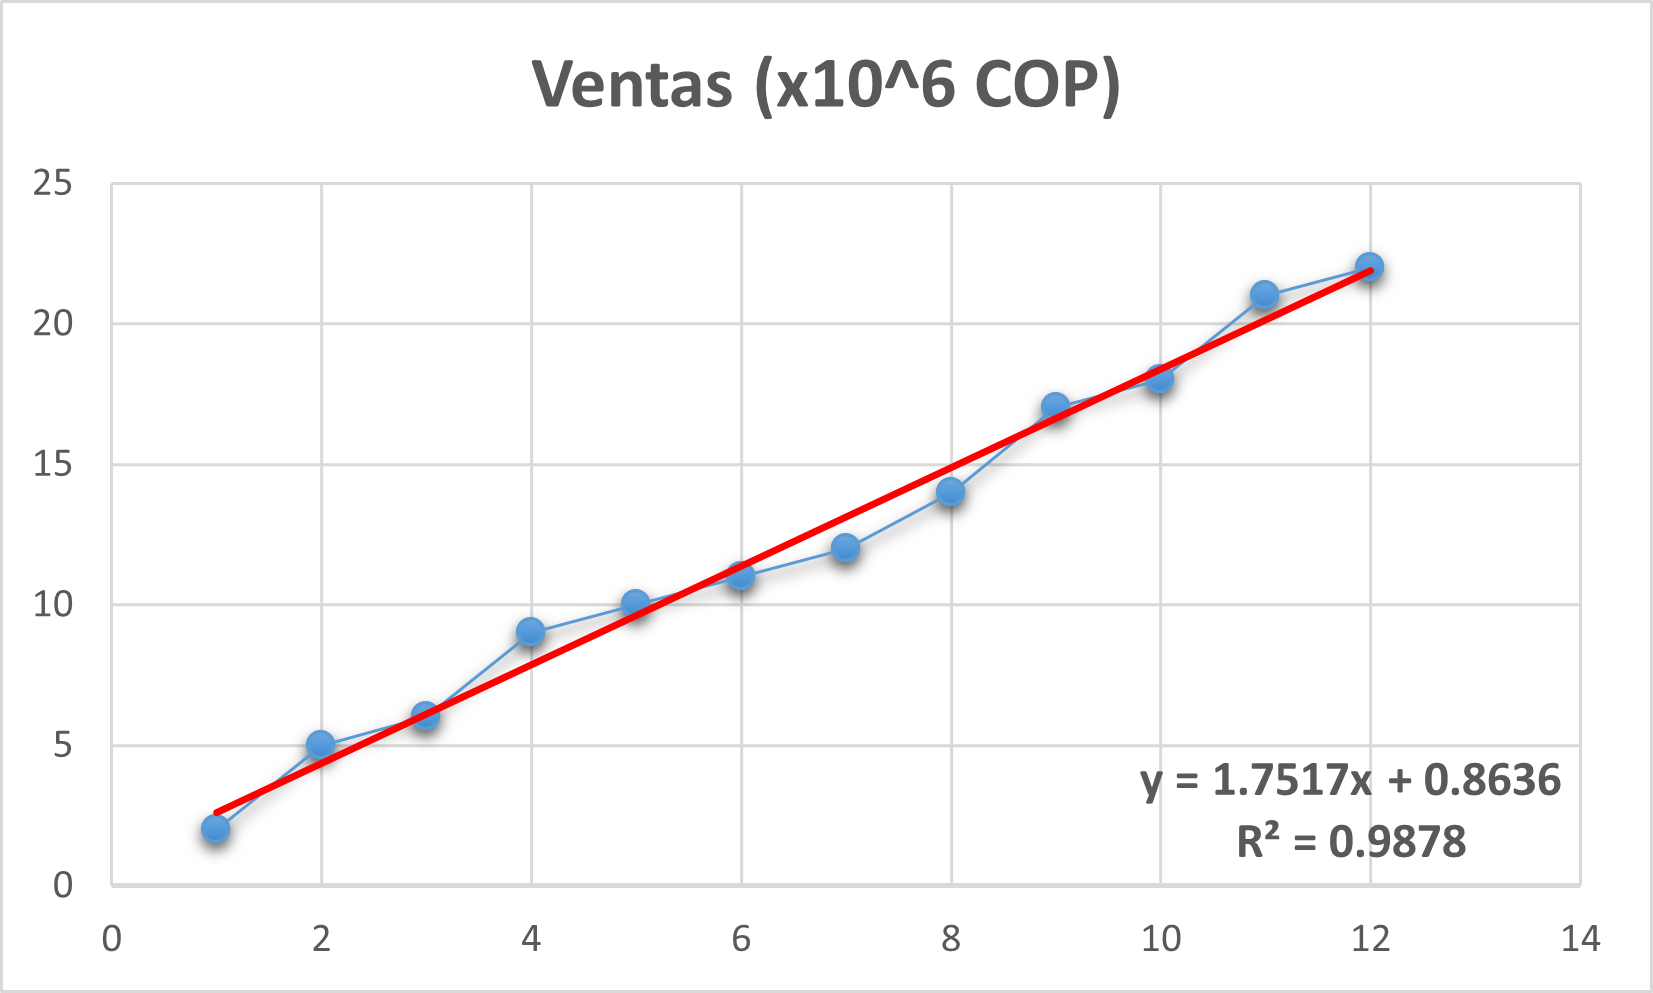
\includegraphics[width=\textwidth]{tendencia.png}
	\caption[short]{Gráfico de tendencia}
	\label{fig:imagen2}
  \end{figure}
  La curva de ventas mensuales tiene picos altos en febrero, abril y septiembre y ventas algo menores en Junio, Julio y octubre. Por otro lado, el análisis de tendencia muestra una línea creciente. Además, el coeficiente de determinación (R cuadrado) indica que la predicción es bastante fiable al ser próximo a uno.
  \newpage
  \bibliographystyle{apacite}
\nocite{*}
\bibliography{instrumentos}
\end{enumerate}
\end{document}